% !TeX document-id = {d8b4925c-2057-42a4-b894-2f1a3f1b6345}
%!TeX TXS-program:compile = txs:///xelatex/[--shell-escape]
\documentclass[aspectratio=169]{beamer}	% TPU recommends 16:9 ratio, 4:3 may require some work with inner theme .sty file

% Style options:
% light --- light theme (default)
% dark --- dark theme
% enlogo --- english TPU logo {default}
% rulogo --- russian TPU logo

\usetheme[light, rulogo]{tpu}		% dark theme used as an example of optional argument

\usepackage[russian]{babel}		%uncomment this to work in russian
\usepackage[utf8]{inputenc}
\usepackage[T2A]{fontenc}

\usepackage{fontspec}

\setromanfont{Brygada1918}[
Path=./fonts/BrygadaFontFiles/,
Extension = .ttf,
UprightFont=*-Regular,
BoldFont=*-Bold,
ItalicFont=*-Italic,
BoldItalicFont=*-BoldItalic
]

\setsansfont{ALSSirius}[
Path=./fonts/ALSSiriusFiles/,
Extension = .otf,
UprightFont=*-Regular,
BoldFont=*-Bold,
%ItalicFont=*-Italic,
%BoldItalicFont=*-BoldItalic
]

\setmonofont{Consolas}[
Path=./fonts/ConsolasFontFiles/,
%Scale=0.85,
Extension = .ttf,
UprightFont=*-Regular,
BoldFont=*-Bold,
ItalicFont=*-Italic,
BoldItalicFont=*-BoldItalic
]

\usepackage[cache=false]{minted}
\usepackage{xcolor} % to access the named colour LightGray
\definecolor{LightGray}{gray}{0.9}
\definecolor{onedarkBckGr}{RGB}{40, 44, 52}

\usemintedstyle[python]{default}
\setminted[python]{
	fontsize=\scriptsize,
	escapeinside=||,
	mathescape=true,
	numbersep=5pt,
	gobble=2,
	linenos=false,
	frame=single,
	framesep=1mm,
	python3=true,
	bgcolor=backcolour,
}

\usepackage{booktabs}	% good looking tables
\usepackage{multicol}	% text in multiple columns, useful for side-by-side text and pictures
\usepackage{hyperref}
%\usepackage{minted}
\usepackage{xcolor}
\definecolor{maroon}{cmyk}{0, 0.87, 0.68, 0.32}
\definecolor{halfgray}{gray}{0.55}
\definecolor{ipython_frame}{RGB}{207, 207, 207}
\definecolor{ipython_bg}{RGB}{247, 247, 247}
\definecolor{ipython_red}{RGB}{186, 33, 33}
\definecolor{ipython_green}{RGB}{0, 128, 0}
\definecolor{ipython_cyan}{RGB}{64, 128, 128}
\definecolor{ipython_purple}{RGB}{170, 34, 255}
\definecolor{linkcolor}{HTML}{0000FF} % цвет гиперссылок
\definecolor{urlcolor}{HTML}{800080} % цвет ссылок
\definecolor{backcolour}{rgb}{0.95,0.95,0.92}

\usepackage{wrapfig}
\usepackage{ragged2e}
\usepackage[nooneline]{caption}
\DeclareCaptionTextFormat{center}{\centering{#1}}
\captionsetup[table]{justification=raggedleft, 
	labelformat=empty,	
	labelsep=endash,  
	textformat=center, 
	position=top, 
	skip=5pt
}

\hyphenpenalty=10000	% i don’t think hyphenation in presentations is a good idea, feel free to change however you like

\title{\LARGE{Системный анализ процессов химической технологии}}
\subtitle{Лекция 1 \\ Операторы управления \\ потоком команд в Python}
\author[]{Вячеслав Алексеевич Чузлов, \\
	к.т.н., доцент ОХИ ИШПР}
\date{\today}

\begin{document}

% notice usage of \titleframe and several other unconventional functions
% the reason being is custom backgrounds on these slides

\titleframe		% title

\tocframe{}		% this custom frame accepts options for ToC



\section{Логический тип данных}
\sectionframe


\begin{frame}[fragile]{Логический тип данных}
\scriptsize
\begin{itemize}

\item Для логического типа данных \mintinline{python}|bool| можно объявлять логические переменные, инициализируя их логическими значениями или присваивая им результат вычисления логических выражений.

\item Логических констант в Python две: \mintinline{python}|True| (истина) и \mintinline{python}|False| (ложь).
\end{itemize}

\begin{minted}[]{python}
|In [1]:| x = True

|In [2]:| y = False

|In [3]:| z = 2 > -1

|In [3]:| print(x, y, z)
|(True, False, True)|
\end{minted}

\vfill
\end{frame}


\section{Операции сравнения}
\sectionframe


\begin{frame}[fragile]{Операции сравнения}
\scriptsize
Логические выражения являются аналогом математической формулы, результатом его вычисления будет одна из двух логических констант~-- \mintinline{python}|True| или \mintinline{python}|False|.

\begin{table}[h!]
%\caption{Операции сравнения}
\centering
\begin{tabular}{|p{.45\textwidth}|p{.45\textwidth}|}
	\hline
	\textbf{Операция} & \textbf{Описание} \\
	\hline
	\mintinline[bgcolor=white]{python}|x < y| & Меньше \\
	\mintinline[bgcolor=white]{python}|x <= y| & Меньше или равно \\
	\mintinline[bgcolor=white]{python}|x > y| & Больше \\
	\mintinline[bgcolor=white]{python}|x >= y| & Больше или равно \\
	\mintinline[bgcolor=white]{python}|x == y| & Равно \\
	\mintinline[bgcolor=white]{python}|x != y| & Не равно \\
	\hline
\end{tabular}	
\end{table}

{\color{tpugreen}\textbullet} Приоритет операций сравнения ниже, чем у арифметических операций:

\begin{minted}{python}
|In [1]:| print(2 + 3 * 5 > 7 / 2 + 3.5)
|True|
\end{minted}
\vfill
\end{frame}


\begin{frame}[fragile]{Операции сравнения}
\scriptsize
Операции сравнения в Python  сравнивают относительные величины своих операндов и возвращают результат логического типа, значение которого обычно используется для выбора следующего действия в более крупном операторе или программе:

\begin{minted}{python}
|In [1]:| 1 < 2       # Меньше
|Out[1]: True|

|In [2]:| 2.0 >= 1    # Больше или равно: число целого типа 1 
   |...:|             # преобразуется к 1.0
|Out[2]: True|

|In [3]:| 3.0 == 3.0  # Значения равны
|Out[3]: True|

|In [4]:| 3.0 != 3.0  # Значения не равны
|Out[4]: False|
\end{minted}
\vfill
\end{frame}


\section{Логические операции}
\sectionframe


\begin{frame}[fragile]{Логическая операция \texttt{not}}
\scriptsize
\begin{itemize}
	\item Унарная логическая операция \mintinline{python}|not| называется логическим отрицанием (<<НЕ>>, инверсия) и указывается перед логическим выражением для получения его противоположного значения.
	
	\item Приоритет операции \mintinline{python}|not| ниже, чем у операций сравнения, поэтому следующее за ней логическое выражение можно не заключать в скобки:
\end{itemize}
\begin{minted}{python}
|In [1]:| print(3 + 5 >= 8)
|True|

|In [2]:| print(not 3 + 5 >= 8)
|False|
\end{minted}
\vfill
\end{frame}


\begin{frame}[fragile]{Логическая операция \texttt{and}}
\scriptsize
\begin{itemize}
	\item Бинарная логическая операция \mintinline{python}|and| называется логическим умножением (логическое <<И>>).
		
	\item Результатом  операции \mintinline{python}|and| будет \mintinline{python}|True| только тогда, когда оба логических выражения будут иметь значения \mintinline{python}|True|, а в прочих случаях результатом будет \mintinline{python}|False|.
\end{itemize}
\begin{minted}{python}
|In [1]:| print(9 + 3 < 10 and 2 + 2 == 4)
|False|

|In [2]:| print(4 + 2 != 0 and 10 * 2 == 20)
|True|
\end{minted}
\vfill
\end{frame}


\begin{frame}[fragile]{Логическая операция \texttt{or}}
\scriptsize
\begin{itemize}
	\item Бинарная логическая операция \mintinline{python}|or| называется логическим сложением (логическое «ИЛИ»).
		
	\item Результатом  операции \mintinline{python}|or| будет \mintinline{python}|False| только тогда, когда оба логических выражения будут иметь значения \mintinline{python}|False|, а в прочих случаях результатом будет \mintinline{python}|True|.
\end{itemize}
\begin{minted}{python}
|In [1]:| print(9 + 3 < 10 or 2 + 2 == 4)
|True|

|In [2]:| print(4 + 2 < 0 or 10 * 2 >= 100)
|False|
\end{minted}
\vfill	
\end{frame}


\begin{frame}[fragile]{Приведение к логическому типу}
\scriptsize
\begin{itemize}
	\item Конструктор типа \mintinline{python}|bool(x)| может использоваться для приведения любого значения к логическому типу (если это значение можно интерпретировать как логический тип). Если аргумент \texttt{*x*} ложь или опущен, то будет возвращено значение \mintinline{python}|False|.
\end{itemize}

\begin{minted}{python}
|In [1]:| print(bool(1), bool(-1.0))
|True True|

|In [2]:| print(bool(0), bool(0.0))
|False False|

|In [3]:| print(bool())
|False|
\end{minted}
\vfill
\end{frame}

\section{Сцепленные операции сравнения}
\sectionframe


\begin{frame}[fragile]{Сцепленные операции сравнения}
\scriptsize
В Python также есть возможность выстраивать цепочки из нескольких операторов сравнения для выполнения проверок вхождения в диапазон. 

Сцепленные сравнения являются краткой записью для более массивных булевых выражений.

\begin{minted}{python}
|In [1]:| x < y > z
|Out[1]: False|

|In [2]:| x < y and y > z
|Out[2]: False|

|In [3]:| 3 < 6 < 9.0 < 12
|Out[3]: True|

|In [4]:| 3 > 6 > 9 > 12
|Out[4]: False|
\end{minted}
\vfill
\end{frame}


\section{Сравнение чисел с плавающей точкой}
\sectionframe


\begin{frame}[fragile]{Сравнение чисел с плавающей точкой}
\scriptsize
Числа с плавающей точкой в логических операциях сравнения могут вести себя неожиданным образом, требуя определенных преобразований для содержательного сравнения:

\begin{minted}{python}
|In [1]:| 0.1 + 1.1 == 1.2  # Кажется, что должно быть True 
|Out[1]: False|

|In [2]:| 0.1 + 1.1  # Близко к 1.2, но не точно: ограниченная точность
|Out[2]: 1.2000000000000002|

|In [3]:| round(0.1 + 1.1, 1) == round(1.2, 1)  # Работает нормально, если 
   |...:|   # выполнить преобразование: функция round выполняет округление, 
   |...:|   # в данном случае до первого знака
|Out[3]: True|
\end{minted}
\vfill
\end{frame}


\section{Оператор \texttt{if}}

\sectionframe	% section title is automatically capitalised

\begin{frame}[fragile]
\frametitle{Оператор \texttt{if}}
\scriptsize
\begin{itemize}
	\item Оператор \mintinline{python}|if| используется для проверки условий: \textbf{если} условие верно, то выполняется блок выражений (называемый <<if-блок>>), \textbf{иначе} выполняется другой блок выражений (называемый <<else-блок>>).
	
	\item Блок <<else>> является необязательным. 
\end{itemize}

\begin{minted}{python}
|In [1]:| if 1:
   |...:|     print('true')
   |...:|
|true|
\end{minted}

Напоминаем, что $1$~-- это \mintinline{python}|True|, таким образом, проверка в операторе всегда проходит. Для обработки ложного результата понадобится добавить часть \mintinline{python}|else|:

\begin{minted}{python}
|In [2]:| if not 1:
   |...:|     print('true')
   |...:| else:
   |...:|     print('false')
   |...:|
|false|
\end{minted}
\vfill
\end{frame}


\begin{frame}[fragile]{Множественное ветвление}
\scriptsize

Рассмотрим пример оператора \mintinline{python}|if|, содержащего все необязательные части:

\begin{minted}{python}
|In [1]:| number = 23

|In [2]:| guess = int(input('Введите целое число: '))

|In [3]:| if guess == number:
   |...:|     print('Поздравляю, Вы угадали,') # Здесь начинается новый блок
   |...:|     print('хотя и не выиграли никакого приза!') # Конец нового блока
   |...:| elif guess < number:
   |...:|     print('Нет, загаданное число немного больше этого.') # Ещё один блок 
   |...:| # Внутри блока Вы можете выполнять любые операторы
   |...:| else:
   |...:|     print('Нет, загаданное число немного меньше этого.')
\end{minted}

\begin{itemize}
	\item  Интерпретатор выполняет операторы, вложенные внутрь первой проверки, которая вернет \mintinline{python}|True|, или часть \mintinline{python}|else|, если все проверки вернули \mintinline{python}|False|. 
	
	\item Части \mintinline{python}|elif| и \mintinline{python}|else| могут быть опущены, а в каждой части допускается указывать более одного вложенного оператора. 
	
	\item Части \mintinline{python}|if|, \mintinline{python}|elif| и \mintinline{python}|else| связываются друг с другом одинаковыми отступами.
\end{itemize}

\end{frame}


\begin{frame}[fragile]{Ограничения блоков: правила отступов}
\scriptsize
\begin{itemize}
	\item Python определяет границы блоков автоматически по \textcolor{extraorange}{\textbf{отступам}} строк.
	
	\item Все операторы с отступами на одинаковое расстояние вправо принадлежат тому же самому блоку кода.
	
	\item Блок заканчивается тогда, когда встречается конец файла или строка с меньшим отступом, и более глубоко вложенный блок просто смещается дальше вправо, чем операторы во включающем блоке.
\end{itemize}
	 
\begin{multicols}{2}

\begin{minted}[linenos=true]{python}
x = 10

if x:
    y = 20
    
    if y:
        print("block 2")
    
    print("block 1")

print("block 0")
\end{minted}
\columnbreak

\centering
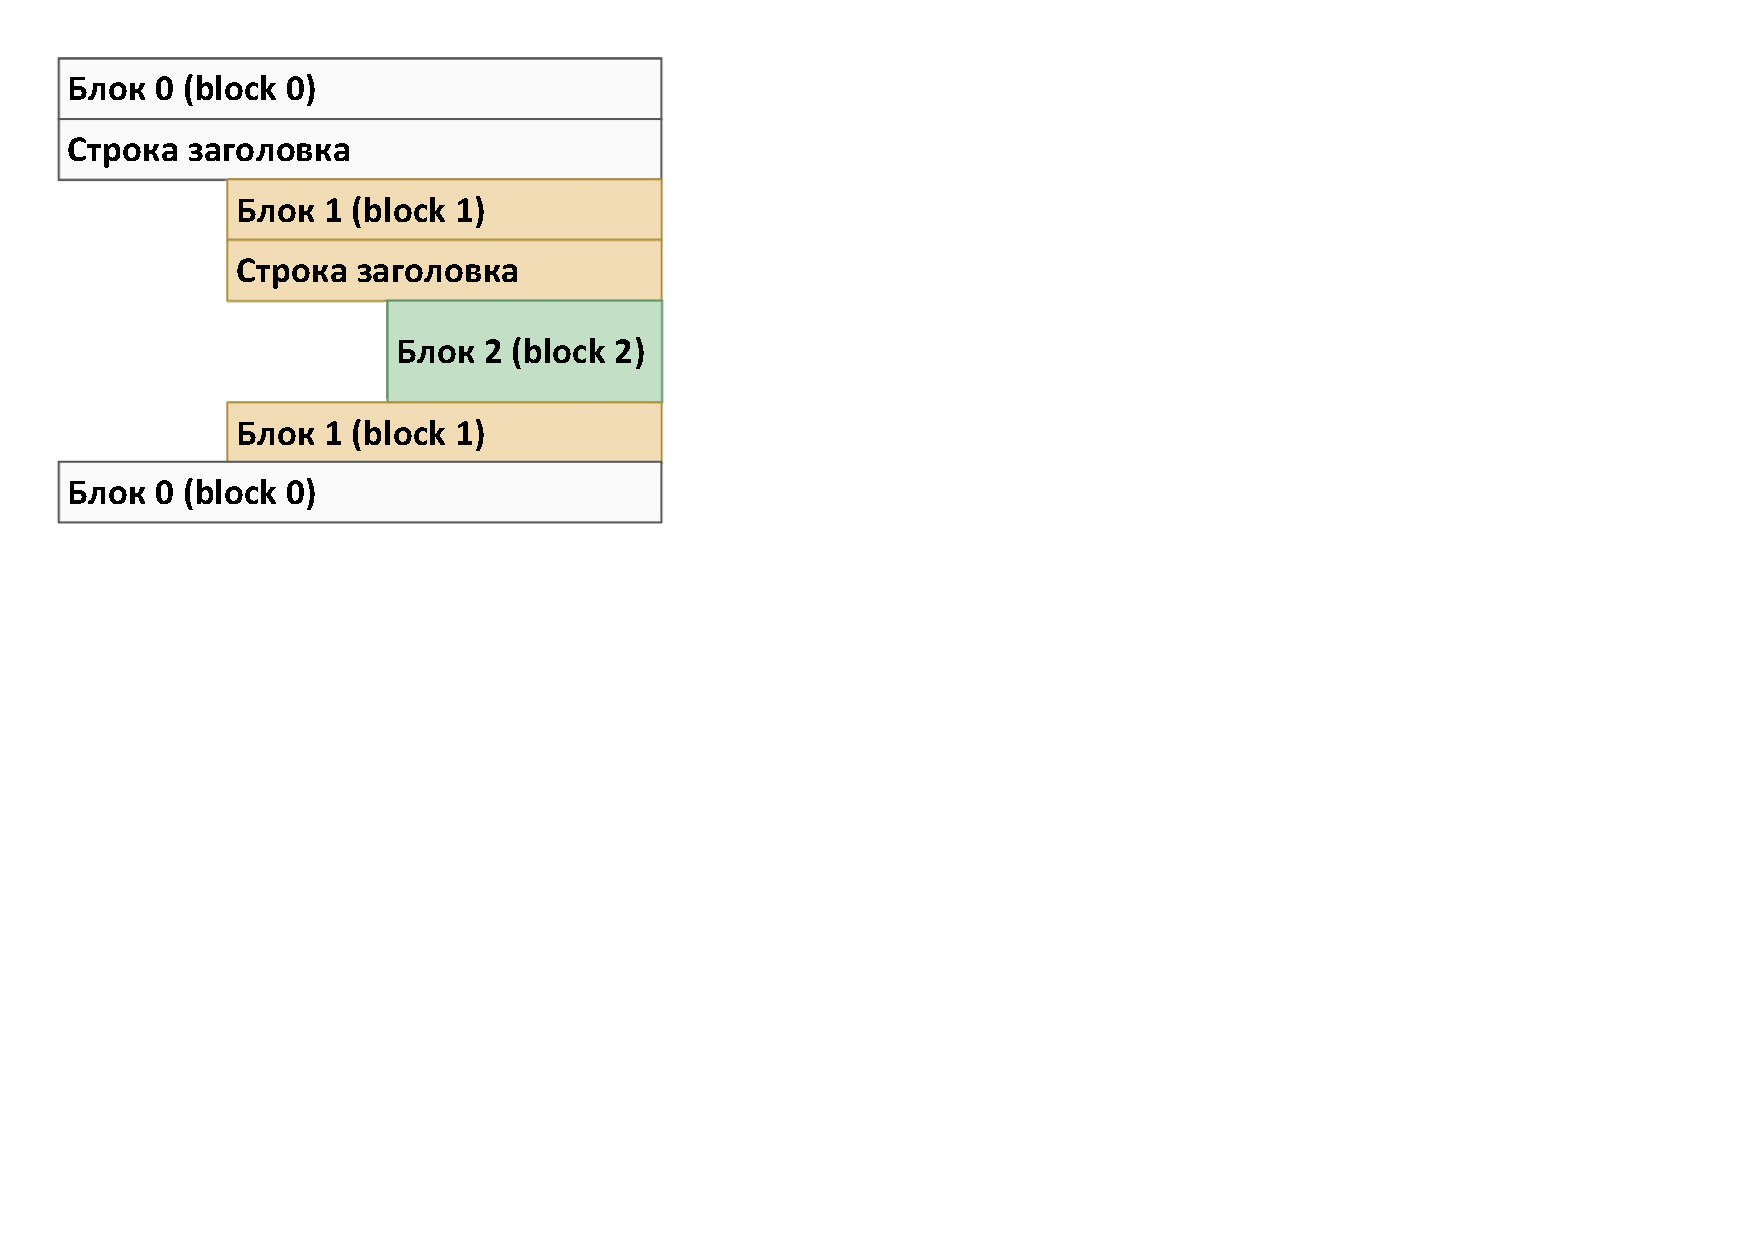
\includegraphics[width=.38\textwidth]{pics/вложенные_блоки_кода}

\end{multicols}	 
\vfill
\end{frame}


\section{Тернарное выражение \texttt{if/else}}
\sectionframe


\begin{frame}[fragile]{Тернарное выражение \texttt{if/else}}
\scriptsize
\begin{itemize}
	\item Зачастую элементы, использованные в операторе \mintinline{python}|if|, достаточно просты, так что распространение такого оператора на четыре строки выглядит излишеством.
	
	\item В других случаях конструкцию подобного рода может понадобиться вложить в более крупный оператор, а не присваивать ее результат какой-то переменной.
	
	\item По указанным причинам в Python был добавлен новый формат условного выражения, который позволяет определить то же самое в одном действии (тернарный оператор).
\end{itemize}

\begin{multicols}{2}

\begin{minted}[linenos=true]{python}
if x:
    a = y
else:
    a = z
\end{minted}

\columnbreak

\begin{minted}[linenos=true]{python}
a = y if x else z
| |
\end{minted}
\end{multicols}
\vfill
\end{frame}


\begin{frame}[fragile]{Тернарное выражение \texttt{if/else}}
\scriptsize
\begin{minted}{python}
|In [1]:| x = 'f' if 10 else 't'  # Числа, не равные нулю, истина

|In [2]:| print(x)
|f|

|In [3]:| x = 'f' if 0 else 't'  # Ноль - это ложь

|In [4]:| print(x)
|t|
\end{minted}
Использовать тернанрый оператор нужно крайне умеренно и только в тех случаях, когда все его составные части относительно просты, иначе предпочтительнее использовать форму полного оператора \mintinline{python}|if| для облегчения его  будущего модифицирования.
\vfill
\end{frame}


\section{Операторы цикла в Python}
\sectionframe


\begin{frame}[fragile]{Операторы цикла}
\scriptsize	
\begin{itemize}
	\item Алгоритмы решения многих задач требуют некоторого количества повторений своих отдельных частей.
	\item Такие повторяющиеся участки называют циклическими, а операторы языка Python, реализующие соответствующие повторения~-- \textcolor{extraorange}{\textbf{операторами цикла}}.
	\item Цикл состоит из \textcolor{extraorange}{\textbf{заголовка цикла}} и \textcolor{extraorange}{\textbf{тела цикла}}.
	\item Заголовок определяет условие прекращения (или выполнения) цикла, а тело цикла содержит операторы, которые нужно повторять.
\end{itemize}

\bigskip	
Операторы цикла в Python:
\begin{enumerate}
	\item Цикл \mintinline{python}|while|
	\item Цикл \mintinline{python}|for|
\end{enumerate}
\vfill
\end{frame}

\subsection{Цикл \texttt{while}}

\begin{frame}[fragile]{Оператор цикла \texttt{while}}

\scriptsize
\begin{multicols}{2}
\begin{itemize}
	\item Оператор \mintinline{python}|while| многократно повторяет блок операторов до тех пор, пока проверка в заголовочной части оценивается как истина.
	
	\item Управление продолжает возвращаться к началу оператора, пока проверка не даст ложное значение. Когда результат проверки становится ложным, управление переходит на оператор, следующий после блока \mintinline{python}|while|.
	
	\item Если проверка оценивается в ложное значение с самого начала, тогда тело цикла никогда не выполнится и оператор \mintinline{python}|while| пропускается.
\end{itemize}
\columnbreak
\centering
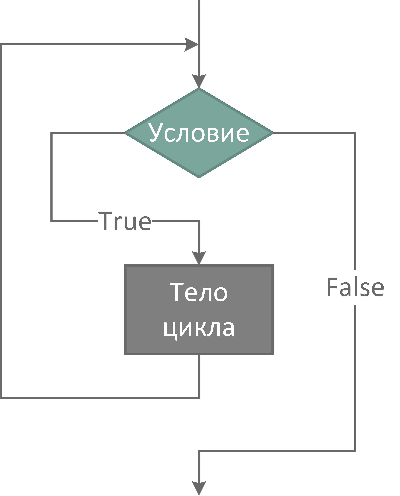
\includegraphics[width=.8\linewidth]{pics/while}
\end{multicols}
\vfill
\end{frame}

\begin{frame}[fragile]{Оператор цикла \texttt{while}}
\scriptsize
Общий формат цикла \mintinline{python}|while|: 

\begin{minted}{python}
while expression:  # Проверка цикла
    operator_1      # Тело цикла
    operator_2
    ...
    operator_n
\end{minted}
Цикл \mintinline{python}|while| можно использовать:
\begin{itemize}
	\item  в математических итерационных алгоритмах для проведения вычислений с заданной точностью;
	\item  при вводе данных, когда их количество заранее неизвестно, а условие завершения ввода определено некоторым введенным значением;
	\item при поиске нужного элемента в какой-либо структуре данных.
\end{itemize}
\vfill
\end{frame}



\begin{frame}[fragile]{Примеры использования цикла \texttt{while}}
\scriptsize
Вывод чисел в диапазоне $[0, 10)$ с шагом $1$:

\begin{minted}{python}
|In [1]:| a, b = 0, 10

|In [2]:| while a < b:
   |...:|    print(a, end='')
   |...:|    a += 1
|0123456789|
\end{minted}
\vfill
\end{frame}


\begin{frame}[fragile]{Примеры использования цикла \texttt{while}}
\scriptsize
\begin{minted}[fontsize=\tiny]{python}
|In [1]:| number = 24

|In [2]:| running = True

|In [3]:| while running:
   |...:|    guess = int(input('Введите целое число: ')) 
   |...:| 
   |...:|    if guess == number:
   |...:|        print('Поздравляем, Вы угадали!')
   |...:|        running = False  # это останавливает цикл while
   |...:| 
   |...:|    elif guess < number:
   |...:|        print('Нет, загаданное число немного больше этого')
   |...:| 
   |...:|    else:
   |...:|        print('Нет, загаданное число немного меньше этого')

|In [4]:| # другие операторы программы
   |...:| print('Завершение.')
|Введите целое число: 12|
|Введите целое число: 24|
|Поздравляем, Вы угадали!|
|Завершение.| 
\end{minted}
\vfill
\end{frame}


\subsection{Цикл \texttt{for}}
\scriptsize
\begin{frame}[fragile]{Оператор цикла \texttt{for}}
	\begin{itemize}
		\item Оператор \mintinline{python}|for...in| также является оператором цикла, который осуществляет итерацию по \textcolor{extraorange}{\textbf{последовательности}} объектов, т.е. проходит через каждый элемент в последовательности.
		
		\item \textcolor{extraorange}{\textbf{Последовательность}}~-- это упорядоченный или неупорядоченный набор элементов.
		
		\item Во многих случаях в заголовке цикла \mintinline{python}|for| используется функция \mintinline{python}|range()|, которая является генератором арифметических прогрессий:
	\end{itemize}

\begin{minted}{python}
|In [1]:| for i in range(10):  # 10 не включительно
   |...:|     print(i, end=' ')
|0 1 2 3 4 5 6 7 8 9|
\end{minted}
\vfill
\end{frame}


\begin{frame}[fragile]{Оператор цикла \texttt{for}}
\scriptsize
Функция \mintinline{python}|range()|~-- генератор арифметических прогрессий:

\begin{minted}{python}
|In [2]:| for i in range(1, 11): # можно задать начальное значение
   |...:|     print(i, end=' ')
|1 2 3 4 5 6 7 8 9 10 |

|In [3]:| for i in range(0, 11, 2):  # также можно менять шаг
   |...:|     print(i, end=' ')
|0 2 4 6 8 10|
\end{minted}
\vfill
\end{frame}


\begin{frame}[fragile]{Вложенные циклы \texttt{for}}
\scriptsize
Операторы цикла \mintinline{python}|for| могут быть вложены друг в друга на произвольную глубину:

\begin{minted}{python}
|In [1]:| for i in range(3):
   |...:|     for j in range(3):
   |...:|         if i != j:
   |...:|             print(i, j, round(1 / (i + j), 2))
0 1 1.0
0 2 0.5
1 0 1.0
1 2 0.33
2 0 0.5
2 1 0.33
\end{minted}
\vfill
\end{frame}


\section{Операторы \texttt{break}, \texttt{continue}, \texttt{pass} и \\ конструкция \texttt{else} цикла}
\sectionframe


\begin{frame}[fragile]{Оператор \texttt{break}}
\scriptsize
Оператор \mintinline{python}|break| выполняет немедленный выход из цикла, т.е. остановку выполнения команд, даже если условие выполнения цикла еще не приняло значение \mintinline{python}|False| или последовательность элементов не закончилась.

\begin{minted}{python}
|In [1]:| while True:
   |...:|     name = input('Enter name: ')
   |...:|     if name == 'stop':
   |...:|         break
   |...:|     age = input('Enter age: ')
   |...:|     print('Hello', name, '=>', int(age) * 2)
|Enter name: John
Enter age: 35
Hello John => 70
Enter name: Julya
Enter age: 24
Hello Julya => 48
Enter name: stop|
\end{minted}
\vfill	
\end{frame}


\begin{frame}[fragile]{Оператор \texttt{continue}}
\scriptsize	
Оператор \mintinline{python}|continue| используется для немедленного перехода в начало цикла.

\begin{multicols}{2}

\begin{minted}{python}
|In [1]:| x = 10

|In [2]:| while x:
   |...:|     x -= 1
   |...:|     # Нечетное? Тогда пропустить
   |...:|     if x % 2 != 0: 
   |...:|         continue  
   |...:|     print(x, end=' ')
|8 6 4 2 0|
\end{minted}

\columnbreak

\begin{minted}{python}
|In [1]:| x = 10

|In [2]:| while x:
   |...:|     x -= 1
   |...:|     # Четное? Тогда выводим
   |...:|     if x % 2 == 0:   
   |...:|         print(x, end=' ')
|8 6 4 2 0|
\end{minted}

\end{multicols}
\vfill
\end{frame}


\begin{frame}[fragile]{Оператор \texttt{pass}}
\scriptsize
\begin{itemize}
	\item Оператор \mintinline{python}|pass|~-- это заполнитель, обозначающий отсутствие действий, используемый в ситуациях, когда синтаксис требует оператора, но нет возможности выполнить что-либо полезное.
		
	\item Данный оператор часто применяется для кодирования пустого тела для составного оператора.
\end{itemize}

К примеру, с помощью \mintinline{python}|pass| можно написать бесконечный цикл, который на каждом проходе ничего не делает:

\begin{minted}{python}
while True:
    pass  # Для прекращения работы нажмите <Ctrl+C>!
\end{minted}
\vfill
\end{frame}


\begin{frame}[fragile]{Конструкция \texttt{else} цикла}
\scriptsize
Полная форма записи циклов \mintinline{python}|while| и \mintinline{python}|for| выглядит следующим образом:

\begin{multicols}{2}

\begin{minted}[linenos=true]{python}
while condition():
    operators

    # Выход с пропуском else
    if exit_test():
        break 

    # Переход к заголовку цикла
    if skip_test():
        continue

# Выполняется, если не было break
else:
    operators
\end{minted}

\columnbreak

\begin{minted}[linenos=true]{python}
for x in collection:
    operators

    # Выход с пропуском else
    if exit_test():
        break 

    # Переход к заголовку цикла
    if skip_test():
        continue

# Выполняется, если не было break
else:
    operators
\end{minted}

\end{multicols}	

Если циклы \mintinline{python}|while| или \mintinline{python}|for| прервать оператором \mintinline{python}|break|, соответствующие им блоки \mintinline{python}|else| выполняться не будут.
\vfill
\end{frame}


\begin{frame}[fragile]{Конструкция \texttt{else} цикла}
\scriptsize
В приведенном примере выполняется проверка, является ли положительное целое число $y$ простым, за счет поиска сомножителей больше 1:

\begin{minted}[linenos=true]{python}
x = y // 2  # Для y > 1

while x > 1: 
    if y % x == 0:  # Остаток от деления
        print(y, "has factor", x)   # Имеет сомножитель
        break  # Пропуск else
    
    x -= 1

else:  # Нормальный выход
    print(y, "is prime")  # Является простым  
\end{minted}
\vfill
\end{frame}


\section{Примеры}
\sectionframe


\begin{frame}[fragile]{Пример~1~-- Fizz Buzz}
\scriptsize
\textbf{Дано:} Положительное целое число (\mintinline{python}|int|) 

\bigskip
<<Fizz buzz>>~-- это игра со словами. Необходимо написать программу, которая принимает положительное целое число и возвращает следующие значения:

\begin{enumerate}
	\item {<<Fizz Buzz>>}, если число делится на 3 и 5;
	\item {<<Fizz>>}, если число делится на 3;
	\item {<<Buzz>>}, если число делится на 5;
	\item Исходное число в остальных случаях.
\end{enumerate}

\bigskip
\textbf{Пример:}
$$
\begin{aligned}
	x = 15 & \qquad \text{результат:} & \quad \text{<<Fizz Buzz>>} \\
	x = 6 & \qquad \text{результат:} & \quad \text{<<Fizz>>} \\
	x = 5 & \qquad \text{результат:} & \quad \text{<<Buzz>>} \\
	x = 7 & \qquad \text{результат:} & \quad 7 \\
\end{aligned}
$$
\vfill
\end{frame}


\begin{frame}[fragile]{Пример~1~-- Fizz Buzz}
\scriptsize
\begin{minted}[linenos=true]{python}
x = int(input('Введите положительное целое число: '))

if not x % 3 and not x % 5:
    print('Fizz Buzz')

elif not x % 3:
    print('Fizz')

elif not x % 5:
    print('Buzz')

else:
    print(x) 
\end{minted}
\vfill
\end{frame}


\begin{frame}[fragile]{Пример~2~-- Вычисление факториала числа n}
\scriptsize
Необходимо написать программу для вычисления $n!$:

$$
	n! = 1 \cdot 2 \cdot 3 \cdot \ldots \cdot (n-1) \cdot n
$$

где $n$~-- положительное целое число.
\vfill
\end{frame}


\begin{frame}[fragile]{Пример~2~-- Вычисление факториала числа n}
\scriptsize
С использованием цикла \mintinline{python}|while|:

\begin{minted}[linenos=true]{python}
n = int(input('Введите положительное целое число: '))

i = 1
f = 1

while i <= n:
    f *= i
    i += 1

print('n! =', f)
\end{minted}
\vfill
\end{frame}


\begin{frame}[fragile]{Пример~2~-- Вычисление факториала числа n}
\scriptsize
С использованием цикла \mintinline{python}|for|:
	
\begin{minted}[linenos=true]{python}

n = int(input('Введите положительное целое число: '))

f = 1

for i in range(1, n + 1):
    f *= i

print('n! =', f) 
\end{minted}
\vfill
\end{frame}


\contactsframe[\Large \textbf{Благодарю за внимание!}]{
	
	
\includegraphics[width=.05\textwidth]{pics/home} \quad Учебный корпус №2, ауд. 136 \\
	
\includegraphics[width=.05\textwidth]{pics/mail} \quad chuva@tpu.ru \\
	
\includegraphics[width=.03\textwidth]{pics/tel} \quad +7-962-782-66-15
}

\end{document}

